\documentclass[nofilelist]{cslthse-msc}
% to show a list of used packages at the end of the document, delete the nofilelist option
%\documentclass{cslthse-msc} 
\usepackage[utf8]{inputenc}
\usepackage[english]{babel}
\usepackage{amsmath}
%\usepackage{amsfonts}
%%\usepackage{amssymb}
\usepackage{amsthm}
%\usepackage{makeidx}
\usepackage{graphicx}
\usepackage[titletoc, header, page]{appendix}
\usepackage{transparent}
\usepackage{natbib}

% used to display the used files at the end. Select nofilelist as a package option to disable this
\listfiles % initialize

%\geometry{showframe}
%better like this?
%\student{Flavius Gruian}{Flavius.Gruian@cs.lth.se}
\students{Nick Persson}{dat14npe@student.lu.se}{Filip Karabeleski}{dat14fka.student.lu.se}

\thesisnumber{LU-CS-EX: 2020-XX} % Birger Swahn will provide this number to you, once the thesis is ready for publication
% default is Master. Uncomment the following for "kandidatarbete"/Bachelor's thesis
%\thesistype{Bachelor}{Kandidatarbete}

%\title{Formatting a Master's Thesis}
\title{Keyword Categorization and Emotion Analysis in Voice Calls}

%\onelinetitle
%\twolinestitle
\threelinestitle
%\fourlinestitle

\subtitle{Subtitle WIP}
\company{Telavox AB}
\supervisors
{Sara Lindgren, \href{mailto:Sara.Lindgren@telavox.com}{\texttt{Sara.Lindgren@telavox.com}}}
{Pierre Nugues, \href{mailto:Pierre.Nugues@cs.lth.se}{\texttt{Pierre.Nugues@cs.lth.se.com}}}
\examiner
{Flavius Gruian,\href{mailto:Flavius.Gruian@cs.lth.se}{\texttt{Flavius.Gruian@cs.lth.se}}}

\date{\today}
%\date{January 16, 2015}

\acknowledgements{
If you want to thank people, do it here, on a separate right-hand page. Both the U.S. \textit{acknowledgments} and the British \textit{acknowledgements} spellings are acceptable.

We would like to thank Lennart Andersson for his feedback on this template.

We would also like thank Camilla Lekebjer for her contribution on this template, as well as Magnus Hultin for his popular science summary class and example document.

Thanks also go to the following (former) students for helping with feedback and suggestions on this template: Mikael Persson, Christoffer Lundgren, Mahmoud Nasser.
}

\theabstract{
This document describes the Master's Thesis format for the theses carried out at 
the Department of Computer Science, Lund University. 

Your abstract should capture, in English, the whole thesis with focus on the problem and solution in 150 words. It should be placed on a separate right-hand page, with an additional \textit{1cm} margin on both left and right. Avoid acronyms, footnotes, and references in the abstract if possible.


Leave a \textit{2cm} vertical space after the abstract and provide a few keywords relevant for your report. Use five to six words, of which at most two should be from the title.
}

\keywords{Machine Learning, NLP, Sentiment Analysis, Keyword Extraction, (style, structure)}

%% Only used to display font sizes
\makeatletter
\newcommand\thefontsize[1]{{#1 \f@size pt\par}}
\makeatother
%%%%%%%%%%

\begin{document}
\renewcommand{\bibname}{References}

\makefrontmatter
\chapter{Introduction}

\section{Background}
Natural language processing (NLP) is a field of study mainly in computer science that deals with analyzing human language in a way that computers can understand and process. According to \citet{ntlk2009}, natural language is used for everyday communication by humans, in contrast to artificial languages such as programming languages and mathematical notations. Since natural languages continuously develop as time goes on and its adherence to structures diminish, it is difficult to define explicit rules to follow. 


The LSTM architecture \citep{ntlk2009} is something....

\begin{itemize}
    \item Förklara vad systemet är
    \item Berätta om företaget Telavox
\end{itemize}

\section{Purpose}
\begin{itemize}
    \item Varför behöver problemet lösas, nytta
\end{itemize}
\subsection{Telavox}
Telavox is a telecommunication company that specializes in business-to-business and business-to-customer unified communication as a service. 
\section{Research questions}
The primary aim of this thesis is to investigate whether or not voice call analysis using NLP can be effective enough to be used as a replacement for manual analysis. 
\textit{What level of precision can be reached with the categorization of keywords from voice calls? }

\textit{How well will our algorithm perform compared to other algorithms carrying out the same measurements?}

\textit{What level of effectiveness can be reached compared to a human manually analyzing the data?} 
\section{Terminology}
NLP, ML, Speech-to-text och (STT), API. Kan också kallas för Glossary and Abbreviations
\section{Delimitations}
Delimitations are choices made by the researcher which should be mentioned. They describe the boundaries that you have set for the study.
\section{Contributions}
Potentialen av applications 
\section{Related work}


\chapter{Approach}

\begin{itemize}
    \item Dataset till input måste följa Googles standard som de följer vid speech to text. 
\end{itemize}

\section{Theory}
NLP technique, categorization, ML, supervised/unsupervised,  
\section{Method} Ta eventuellt bort
Word level one hot encoding, kanske relevant, avgör beroende på hur mycket mer vi behöver skriva.
\section{Implementation} Ta eventuellt bort
Overfitting \\
Data Augmentation \\
importance of finding the correct data-sets \\
\section{Bibtesting, will be removed}
\citep{emotionlinesdataset} \\
\citep{franoischollet2017learning}\\
\citep{beaver2020towards}
\chapter{Speech-to-text}
Vi antar att det är 2 speakers i samtalet, nämn för- och nackdelar. Ta med i limitations
Vi har endast stöd för engelska pga limits i datamängd, dokumentation. 
Google diarization är i Beta.
Använda kategoriserade ord i Googles STTs speechContexts och därefter använda ML igen för att få högre precision på kategorisering. 
Sample rates 8000 vs 48000 t.ex.

Cased eller uncased? Hur fungerar google speech-to-text med cased/uncased?

\chapter{Keyword Extraction}
\chapter{Emotion Analysis}
6 eller 4 känslor
Sentiment analysis, varför valde vi inte det?


\chapter{Evaluation}

\section{Results}
\section{Discussion}


\chapter{Conclusions}



% Should use consistent formatting when it comes to Names ("FirstName LastName", or "F. LastName")
%\printbibliography
\makebibliography{MyMSc}

\begin{appendices}
\chapter{Dummy Appendix}






% display used packages information unless nofilelist is used in the cslthse-msc package option
\printfilelist

%make sure we're on even page with the pop-sci
\checkoddpage
\ifoddpage
\else
   \newpage
   \thispagestyle{empty}
   \mbox{ }
\fi
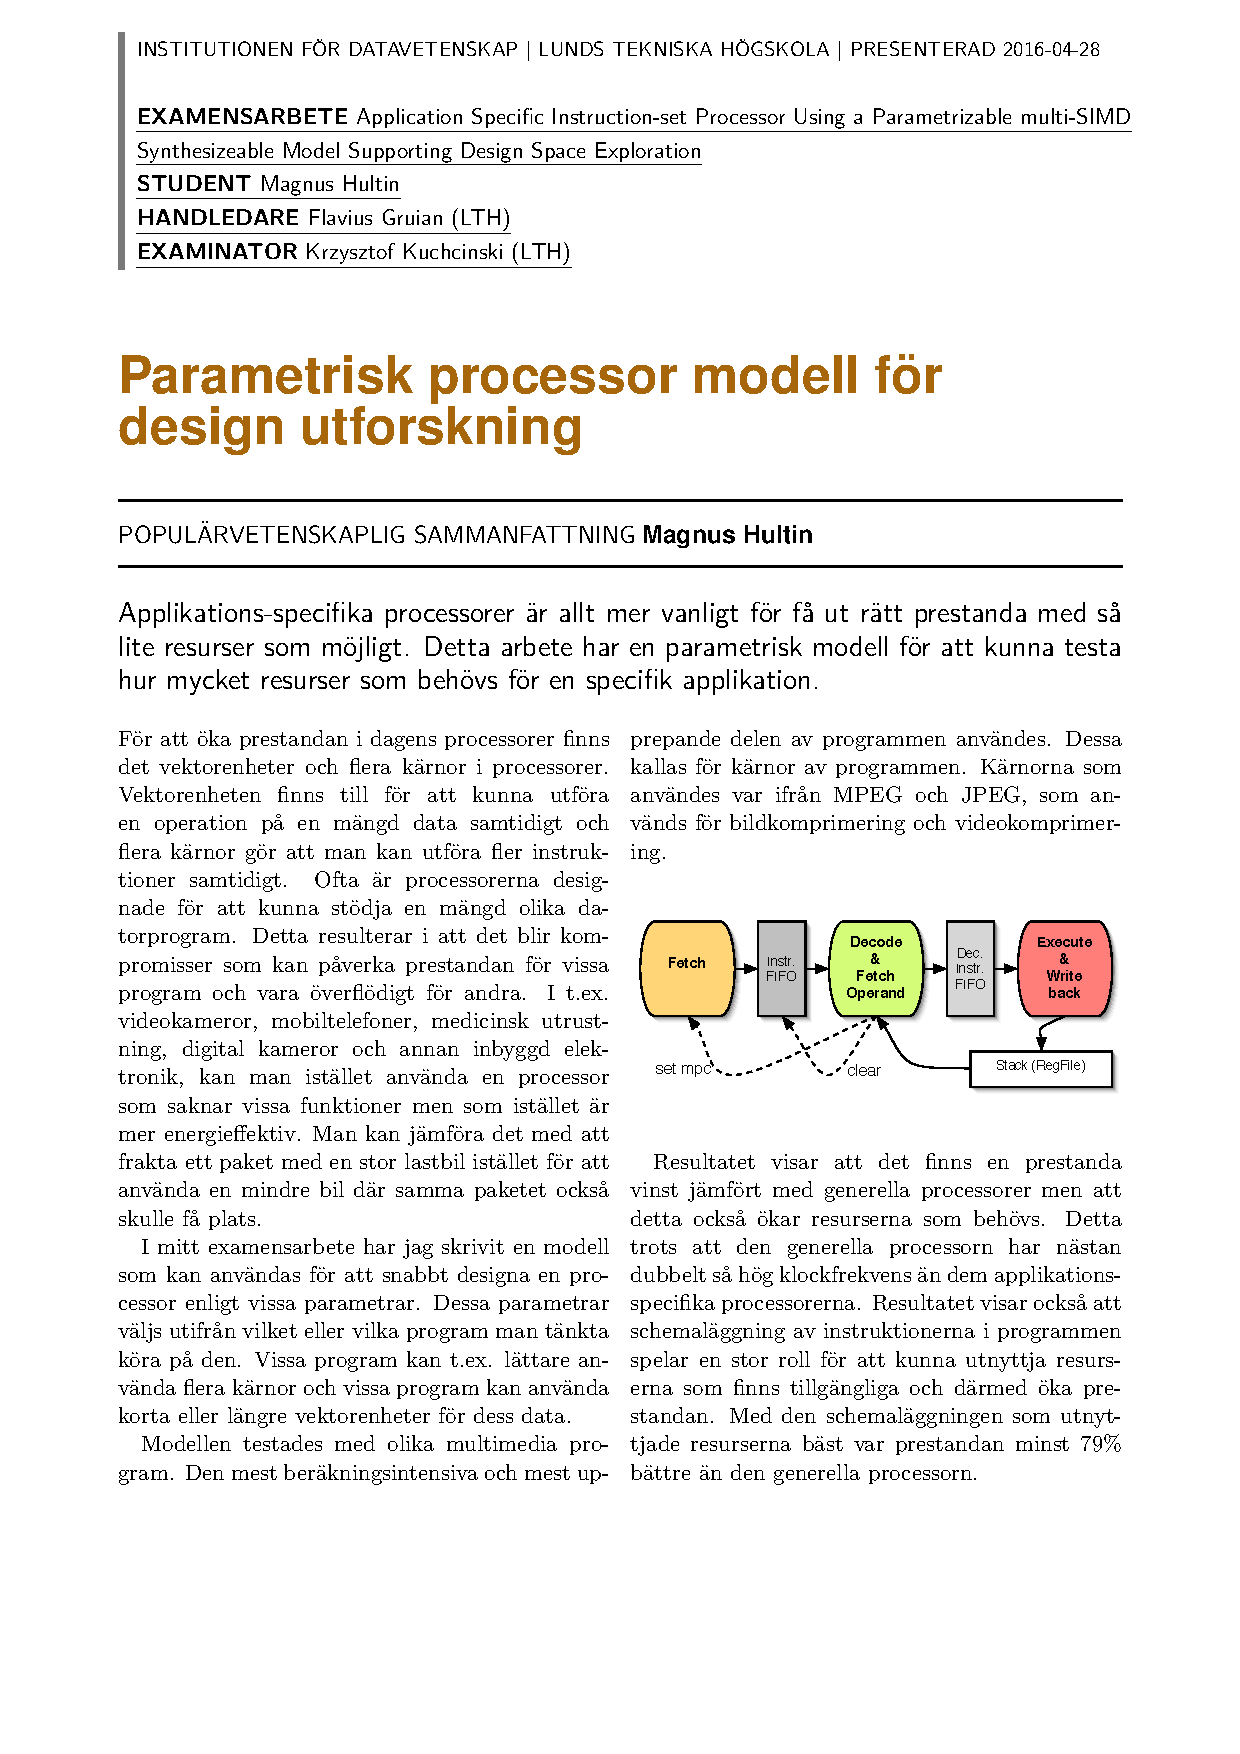
\includepdf[pages={1}]{popsci/popsci.pdf}
\end{appendices}

\end{document}